%File: AAAI-inst.tex
% support for LaTeX is provided by AAAI, and these instructions
% and the accompanying style files are NOT guaranteed to work.
% If the results you obtain are not in accordance with the 
% specifications you received in your packet (or online), you
% must correct the style files or macro to achieve the correct
% result. 
%

%
% The instructions herein are provided as a general guide for 
% experienced LaTeX users who would like to use that software
% to format their paper for an AAAI Press proceedings or technical
% report or AAAI working notes. These instructions are generic. 
% Consequently, they do not include specific dates, page charges, and so forth. 
% Please consult your specific written conference instructions for 
% details regarding your submission.
%
% Acknowledgments
% The preparation of the \LaTeX{} and Bib\TeX{} files that
% implement these instructions was supported by 
% Schlumberger Palo Alto Research, AT\&T Bell
% Laboratories, Morgan Kaufmann Publishers, and AAAI Press.
\documentclass[letterpaper]{article}
\usepackage{aaai}
\usepackage{times}
\usepackage{helvet}
\usepackage{courier}
\usepackage{amsfonts}
\usepackage{mathtools}% Loads amsmath
\usepackage{graphicx}

\usepackage{algorithm}
\usepackage[noend]{algpseudocode}

\usepackage{booktabs}
\usepackage[normalem]{ulem}
\useunder{\uline}{\ul}{}

\makeatletter
\def\BState{\State\hskip-\ALG@thistlm}
\makeatother

\begin{document}
% The file aaai.sty is the style file for AAAI Press 
% proceedings, working notes, and technical reports.
%
%\title{Model Selection for Causal Inference using Deep Neural Networks}
% TODO: What about 
%\title{Architecture Learning for Deep Counterfactual Networks}
\title{Architecture Learning of Deep Neural Networks for Counterfactual Inference}
\author{Author One, Author Two, Author Three\\
Authors Details\\
Authors Email}
\maketitle


\begin{abstract}
\begin{quote}
We propose a novel approach for automatically inferring appropriate architectures of deep neural networks for the task of counterfactual inference over observational data. The individualised causal effect of an intervention or treatment is modelled in terms of  a multi-task learning  problem using a deep neural network which consists of a number of layers that are shared among the factual and counterfactual outcomes and a number of outcome-specific layers. Our approach enables automatically selecting an appropriate architecture (i.e. number of shared and outcome-specific layers) by exploiting inferred characteristics of the dataset such as the propensity score, the extend of shared  complexity between the two outcomes and the outcome-specific complexities. This way, we achieve an efficient method of model-selection while avoiding computationally expensive hyper-parameter searches over the space of possible architectures.  
We conduct experiments on a synthetic dataset allowing us to parametrize and fully control the characteristics of the data before applying our approach to a real-world observational study for which we infer the characteristics in order to derive an appropriate architecture. As shown in the experiments, our method outperforms the state-of-the-art.
 
\end{quote}
\end{abstract}


\section{Introduction}
The technological advancements of recent years have resulted in an increasing availability of data in various fields such as healthcare, education, and economics. This data can be used to make predictions concerning unseen data points on the basis of statistical models. When dealing with observational studies, we are often particularly interested in the task of predicting the individualised treatment effect that certain intervention has on a given subject or context. In the case of electronic health records, for instance, a dataset typically consists of a set of patients each with individual features, a treatment assignment indicator (i.e. whether or not they received the treatment), and an observed outcome which we call the \emph{factual outcome}. The quantity we are interested in is the \emph{counterfactual outcome} (i.e. the outcome had the patient received a different treatment assignment) because it allows us to compute the individualised treatment effect helping us make informed decision during treatment planning. % TODO Add sources


% TODO Check how much I can take from Ahmed's Sentence
Classical works have focused on estimating average treatment effects through variants of propensity score matching \cite{rubin2011,austin11,Abadie2016,rosenbaum83,rubin73}. More recent works tackled the problem of estimating individualised treatment effects using representation learning \cite{sontag1,sontag2}, Bayesian inference \cite{hill}, and standard supervised learning \cite{wager}. \\

Recent works have shown that the problem can be effectively framed in terms of a multi-task learning problem using deep neural networks \cite{propensity-dropout}. The network has a set of layers that are shared among both the factual and the counterfactual outcomes and a number of outcome-specific layers. However, the questions of how to select an appropriate architecture (i.e. the number of shared layers, and the number of outcome-specific layers) may drastically influence the expressiveness and computational complexity of the model and remains an open challenge. While there are various general approaches for model selection and architecture learning in neural networks, they do not make use of the specific nature of causal inference. % TODO Quote Model selection papers
 \\

In this paper, we propose a novel approach for automatically learning appropriate architectures of deep neural networks for the task of counterfactual inference over observational data. This is achieved by exploiting inferred characteristics of the dataset such as the propensity score, and the "shared complexity" among the different outcomes and the difference between the outcome surfaces. For instance, if one of the outcomes follows a much more complex function than the other, this should be reflected in a potentially asymmetric architecture which utilises a higher number of outcome-specific layers for the more complex outcome. 


%This is my introduction
%* What is counterfactual inference
%* Why does it matter?
%* Application areas
%
%* What is deep learning? 
%* Why is it appropriate for causal inference
%* We use multi-task learning
%
%* Which datasets? 
%
%* Model selection for deep learning is difficult
%* There are various methods, but they don't exploit the specific nature of causal inference
% TODO: Do I need a dedicated Related Works Section or is implicit in the introduction? 
%\section{Related Works}
%% TODO Check related works
%* Deep Learning
%* Model selection (Optimal Brain Damage, Optimal Brain Surgeon) 
%* Causal Inference using Deep Neural Nets (Sontag et al)
%* Our other ICML paper


\section{Problem Formulation}
% TODO Check if it's okay that this is so similiar to previous paper
% TODO cite Rubin 2011
We represent each subject $i$ in our population  with a $d$-dimensional feature vector $X_i \in \mathcal{X}$, and two \emph{potential outcomes} $Y_{i}^{(1)}, Y_{i}^{(0)} \in \mathbb{R}$ which are drawn from a distribution $(Y_{i}^{(1)}, Y_{i}^{(0)}) \mid X_i = x \sim \mathbb{P}(\cdot \mid X_i = x)$. This way, the \emph{individualised treatment effect} for subject $i$ can be expressed as 

\[
T(x) = \mathbb{E}[Y_{i}^{(1)} - Y_{i}^{(0)} \mid X_i = x] . \tag{1} \label{eq:ite}
\]

Given this definition, the objective is to approximate the function $T(x)$ using an observational dataset $\mathcal{D}$ consisting of $n$ independent samples. Each sample is comprised of a tuple $ \langle X_i, W_i, Y_{i}^{(W_i)} \rangle$, where $X_i$ represents the subject's features, $W_i \in \{0,1\}$ the treatment assignment indicator, and $Y_{i}^{(W_i)}$ and $Y_{i}^{(1 - W_i)}$ the respective \emph{factual} and \emph{counterfactual} outcome. 
The treatment assignment is a random variable depending on the subjects' features, i.e. $W_i \not \perp X_i$. The assignment reflects a domain-specific policy which can be captured in terms of the probability $p(x) = \mathbb{P}(W_i = 1 \mid X_i = x)$ called the \emph{propensity score}. \\

% TODO Quote Rubin
% TODO Describe multi-task learning
% TODO What is the formalism of what we want to show here? 
%
%* What does Model Selection mean? 
%* Which objective function are we trying to optimise
We are following the approach of \cite{propensity-dropout}
% TODO CITE our own paper
and are using a \emph{deep counterfactual network} (DCN) to infer $T(x)$ from $\mathcal{D}$. The DCN treats the problem as a multi-task learning problem using a deep neural network with an architecture illustrated in figure \ref{fig:dcn-architecture}.
The network uses a number $L_s$ of shared layers, a number $L_{i,0}$ of idiosyncratic (outcome-specific) layers for the \emph{treated outcome}, and a number $L_{i,1}$ for the \emph{control outcome}. \\

We are interested in learning an appropriate architecture of the DCN, i.e. coming up with suitable values for $L_s$, $L_{i,0}$, and $L_{i,1}$. 


\begin{figure}
	\centering
	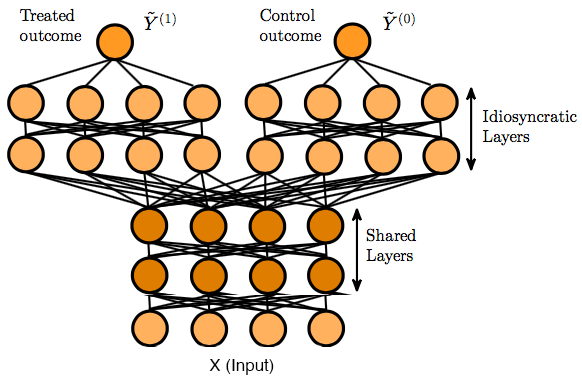
\includegraphics[width=0.5\textwidth]{img/fig-dcn-architecture.png}
	\caption{DRAFT: Architecture of a Deep Counterfactual Network (DCN). Objective is to learn appropriate values for number of different layers (here $L_s = L_{i,0} = L_{i,1} = 2$).}
	\label{fig:dcn-architecture}
\end{figure}

\section{Architecture Learning}
We propose a novel approach of automatically learning a suitable architecture for the DCN by exploiting relevant characteristics of the dataset which are specific to the problem of causal inference. These characteristics such as the propensity score, the shared complexity of the response surfaces, and the individual complexity of each outcome function, can be inferred from the data to inspire a suitable architecture. This way, we achieve an efficient method of model-selection while avoiding computationally expensive hyper-parameter searches over the space of possible architectures. \\

The approach is based on the observation that certain architectures are more suitable than others for the task of counterfactual inference. In particular, it can be shown empirically (see appendix)
% TODO Add apendix
 that the best-performing architectures consistently follow specific empiric ratios between the number of shared and total layers, and the respective idiosyncratic and total layers. The optimal ratios are not static, however, but depend on specific characteristics of the dataset. Once these characteristics are known, we can directly compute the desired number of layers and obtain a suitable architecture without the need to perform a hyper-parameter search.

In the following, we will discuss each characteristic in detail, including its intuition and formalisation. We describe how the characteristic can be inferred from the data and how it can be used to inform the architecture of the DCN.

\begin{figure}[]
	\centering
	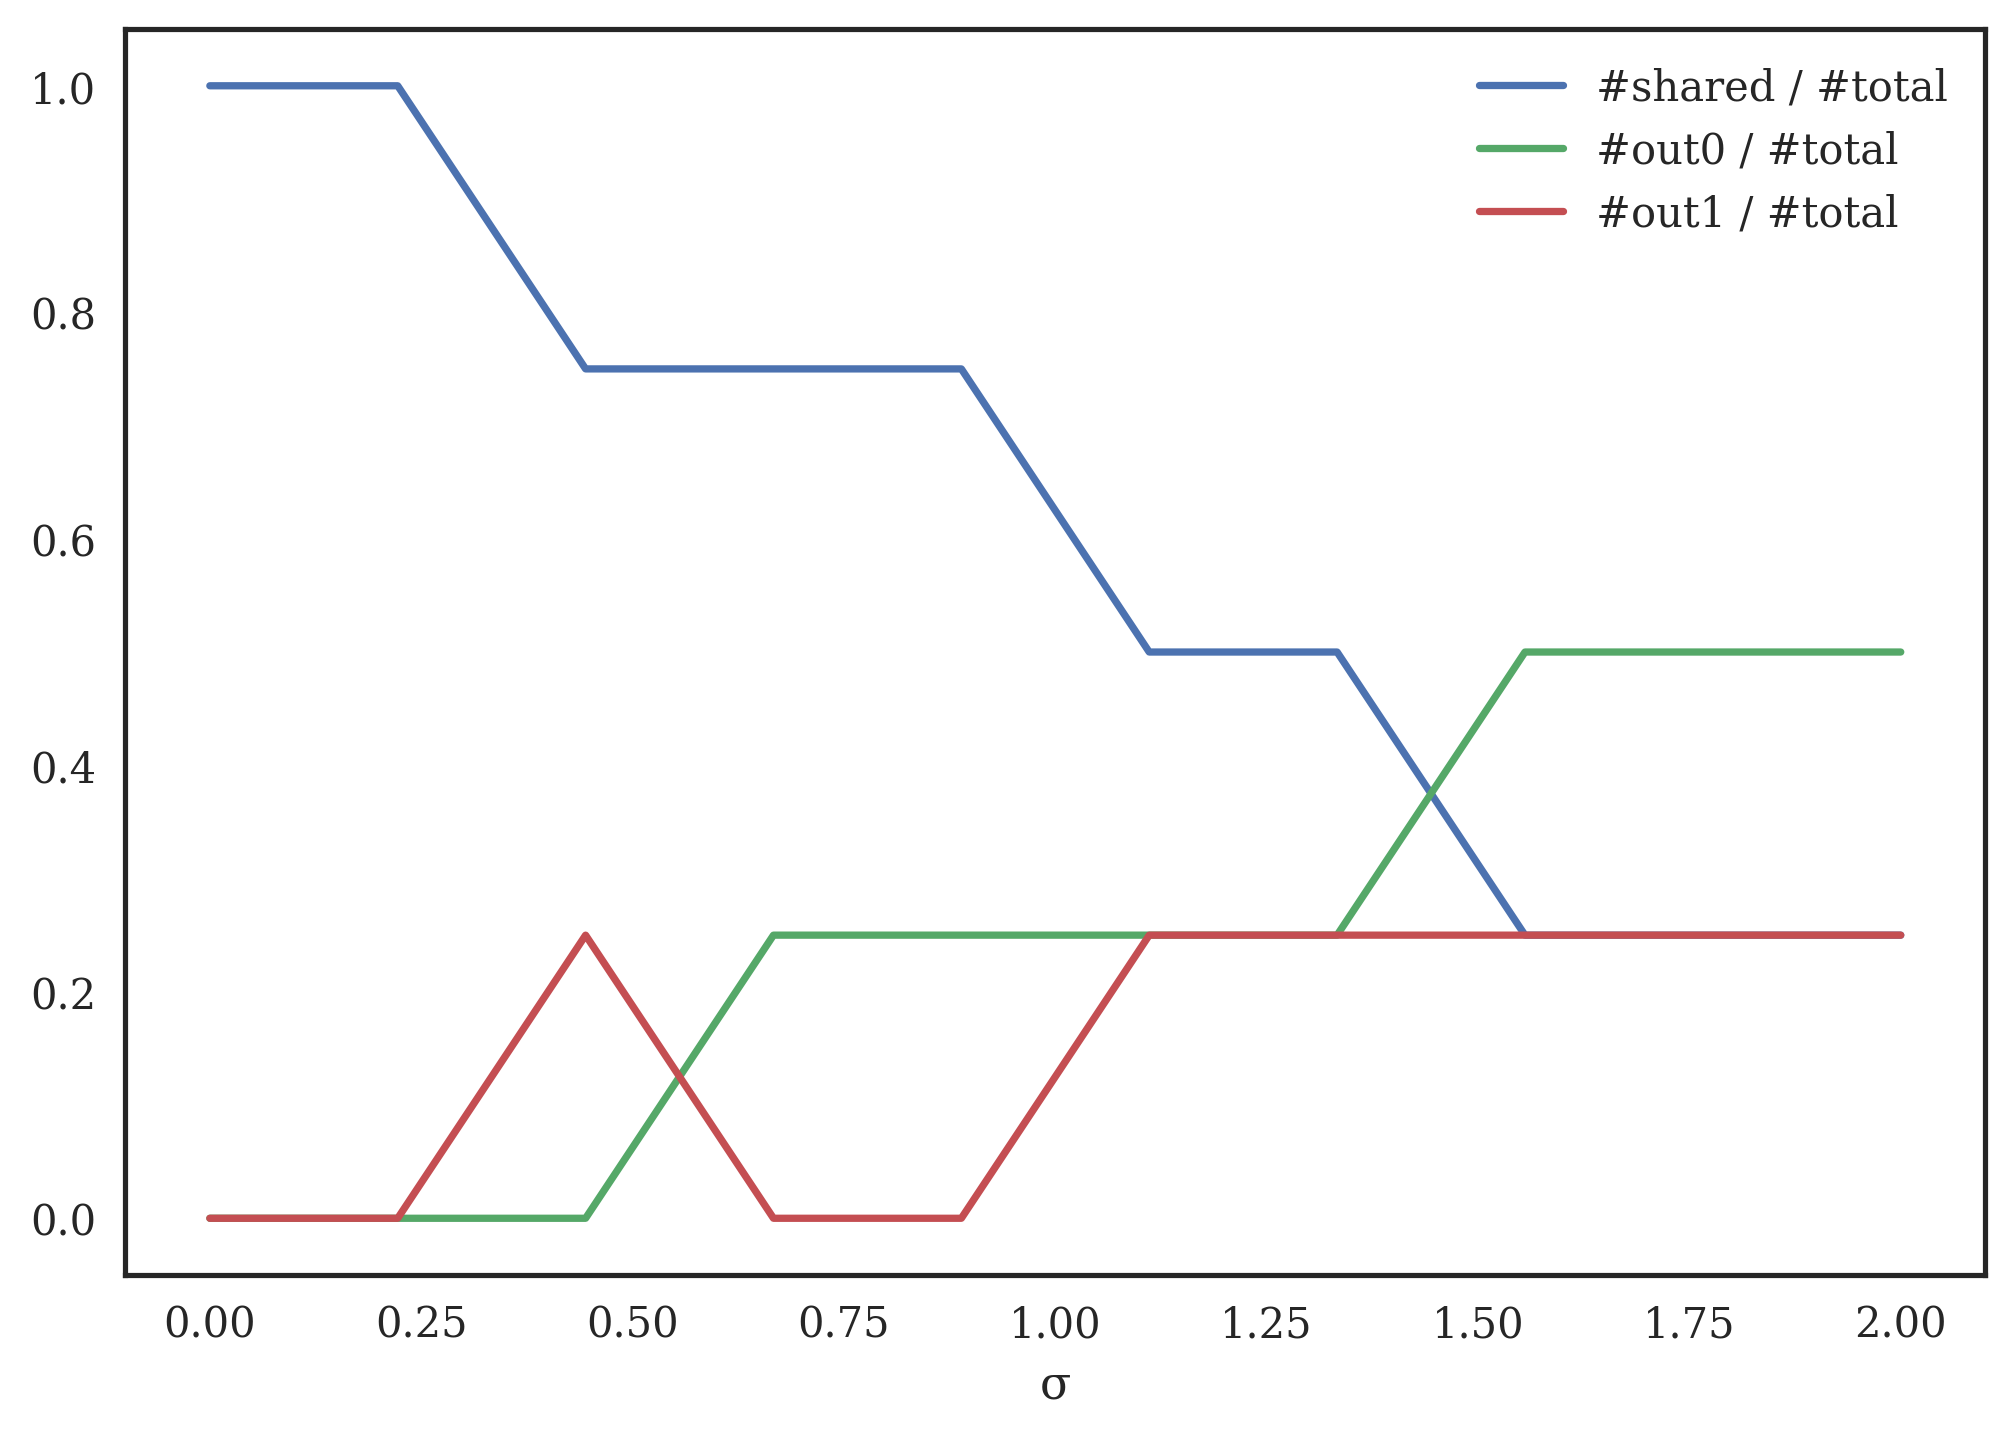
\includegraphics[width=0.4\textwidth]{img/fig-syn-sigma}
	\caption{DRAFT: Influence of similarity parameter $\sigma$ on the learnt optimal architecture with $L_\text{total} = 4$ fixed. }
	\label{fig:syn-sigma}
\end{figure}



\subsection{Relevant Characteristics}
For the problem of counterfactual inference, we have identified the following main characteristics of the data. 

\subsubsection{(a) Selection Bias}
Each dataset can be considered a partition  of subjects into treated and untreated (control) subjects depending on their treatment assignment indicator $W_i$ as described in the previous section. Governed by the underlying treatment policy the dataset might be heavily imbalanced and skewed towards a specific treatment. 
Intuitively, this potential imbalance is relevant for our model because we might profit from a corresponding asymmetric architecture, i.e. a model where the number of outcome-specific layers differ from each other. 

Formally, the selection bias $\mathbf{B}$ can be quantified in terms of the average propensity score 
$$
\mathbf{B} = \frac{1}{n} \cdot \sum \limits_{{i=0}}^{n-1}  \mathbb{P}(W_i = 1 \mid X_i).
$$

The individual propensity scores can be estimated from the dataset using a neural network for which we treat the prediction of the treatment assignment as a binary classification problem in supervised learning. 



\subsubsection{(b) Similarity of  Outcome Response Surfaces}
The different outcome functions of the treated and untreated subjects can be conceptualised in terms of a shared part governed by features and their correlations that are mostly the same for both outcomes and an outcome-specific part that is inherently different. \\

Intuitively, if the outcome functions are potentially complex but rather similar to each other, this should be reflected in a high number of shared layers in the network in contrast to a relatively low number of outcome-specific layers. \\

Formally, we can model the different outcomes as functions
\begin{align}
\label{eqn:outcome-functions}
\begin{split}
f_1(X_i) =  \underbrace{g(X_i, \lambda^{(1)})}_{\text{shared}} +   \beta_1 \cdot \underbrace{ exp(h_1(X_i, \mu^{(1)}))}_{\text{outcome-specific}}
\\
f_0(X_i) = \overbrace{g(X_i, \lambda^{(0)})} +  \beta_0 \cdot \underbrace{exp(h_0(X_i, \mu^{(0)}))}_{\text{outcome-specific}}
\end{split}
\end{align}


where $g$ represents a common function and $h_0, h_1$ are outcome-specific (e.g. polynomial functions of different degrees). The relative weight of the shared part in comparison to the outcome-specific part is captured by $\beta_0, \beta_1 \in \mathbb{R}$ (see below). In this model, the vectors $\lambda^{(1)}, \mu^{(1)}$ represent the coefficients of a specific response surface for the factual outcome whereas we model their counterfactual counterparts as
\begin{equation}
\label{eqn:mu_and_sigma}
\lambda^{(0)}_i \sim \mathcal{N}(\lambda^{(1)}_i, \sigma)  \hspace{1cm} \mu^{(0)}_i \sim \mathcal{N}(\mu^{(1)}_i, \sigma).
\end{equation}


This way, we can use the parameter $\sigma \in \mathbb{R}^0$ to formalise a measure of similarity $\mathbf{S} = \sigma$ between the two outcome surfaces. A low sigma corresponds to a high similarity which should be reflected in a large amount of shared layers, whereas an increasing sigma should result in a smaller proportion of shared layers. \\

There are multiple ways to estimate $\mathbf{S}$ for a new dataset. In our approach, we train two separate feed-forward neural networks -- one exclusively for the treated subjects and one exclusively for the untreated subjects. After training, we compare the coefficients according to equation ($\ref{eqn:mu_and_sigma}$) and get an estimate for $\mathbf{S}$. 
%TODO More precisely. What is the architecture of the networks? How do they relate to the metric above? How do we compare the coefficients. 
%* What do we mean by that? \\ % TODO Or should that go to the formalism section? 
%* What does it depend on? \\ 
%* How do we measure it? \\
%* How should it be reflected in the layers? \\
%* How does it influence the architecture? \\
%* Qualitatively? Quantitatively? \\
%* shared / total or out1 / total, out2 / total ? \\
%\emph{Draft: How can we learn this from the data in a non-synthetic scenario?} \\
%\emph{Draft: How does it inform the architecture (number of layers) concretely?}

\subsubsection{(c) Individual Complexity of each Response Surface}
In addition to the complexity that is shared across both response surfaces, the outcomes normally possess an individual part that is outcome-specific and follows a completely different type of function. For instance, one of the outcomes might be linear whereas the other outcome might be a polynomial function of a higher degree. 
Intuitively, the outcome with the more complex function should have a higher number of outcome-specific layers in our model in order to capture the more complex correlations between the features, leading to an overall asymmetric architecture. 

In order to formalise the outcome-specific complexity, we use the same model for the outcome functions as defined in equations (\ref{eqn:outcome-functions}). This time we focus on the parameters $\beta_0, \beta_1 \in \mathbb{R}$ which can be used to model the relative weight that is put on the outcome-specific part in comparison to the shared part. A low value for $\beta_0$ or $\beta_1$ corresponds to a simpler individual response surface whereas higher values lead to more complex functions.  This way, we achieve a measurement of the individual outcome-complexities $\mathbf{C_0}, \mathbf{C_1}$.
% TODO How do I learn this? 

%%
%%where $g$ represents a common function and $h_0, h_1$ represent polynomial functions of different degrees (e.g. linear vs. quadratic). This way, we can use the parameters $\beta_0, \beta_1 \in \mathbb{R}^0$ to model the relative importance of the individual outcome-specific complexity in relation to the shared one.  \\ \\
%
%%* What do we mean by that? \\ % TODO Or should that go to the formalism section? 
%%* What does it depend on?  \\
%%* How do we measure it? \\
%%* How should it be reflected in the layers? \\
%%* How does it influence the architecture? \\
%%* Qualitatively? Quantitatively? \\
%%* shared / total\\
%\emph{Draft: How can we learn this from the data in a non-synthetic scenario?} \\
%\emph{Draft: How does it inform the architecture (number of layers) concretely?}

%\subsection{Deriving a suitable Architecture for the DCN} 
%* Once we are able to quantify these characteristics, what do we do with it? \\ 
%* What is the relationship between these characteristics and an appropriate architecture? 

% TODO: Do we need to train the model (e.g. using characteristics-based objective function). If so, this would be the section:
%\subsection{Training the Model}
%* How does the training algorithm work?
%* How do we compute the quantities / characteristics / statistics? 
%* Show pseudocode of algorithm


\subsection{Algorithm}
Having defined and formalised the relevant characteristics of the dataset, we can derive a suitable architecture for your models as described in algorithm \ref{fig:algorithm}. \\

First, we estimate the appropriate 


\begin{algorithm}
	\caption{Architecture Learning}\label{fig:algorithm}
	\begin{algorithmic}[1]
		
		\Procedure{Architecture Learning for DCN}{} \\
		\textbf{Input:} Dataset $\mathcal{D}$, $L_{total}$  
		\State \emph{\# Learn Characteristics from dataset}
		\State $\ \tilde{\mathbf{B}} \gets \textit{estimate selection bias (a)}$
		\State $\ \tilde{\mathbf{S}} \gets \textit{estimate response surface similarity (b)}$
		\State $\ \tilde{\mathbf{C_0}}, \tilde{\mathbf{C_1}} \gets \textit{estimate individual complexity (c)}$\\
		\State \emph{\# Derive Architecture}
		\State $\ \tilde{L_s} \gets \textit{Learned via propensity network}$
		\State $\ \tilde{L_{i,0}} \gets \textit{Learned via separate network}$
		\State $\ \tilde{L_{i,1}}, \tilde{\beta_1} \gets \textit{Learned via separate network}$ \\
		\textbf{Return:} $L_s, L_{i,0}, L_{i,1}$ 

		\EndProcedure
	\end{algorithmic}
\end{algorithm}


\section{Experiments}
The experiments are conducted on two different datasets. Firstly, we use a synthetic model which allows us to parametrise and fully control the characteristics mentioned in the previous section. This gives us the power to investigate how the different characteristics influence the performance of the learnt architecture.
Secondly, we run the experiments on the \emph{UNOS} dataset % TODO Cite UNOS
(consisting of information regarding patients who underwent an organ transplantation) to show how our approach generalises to a real-world dataset for which we do not have access to the characteristics directly but have to infer them from the data in order to learn a suitable architecture. 
In both cases, we compare the performance of a DCN whose architecture was learnt by our approach to a generic DCN and a number of other baseline approaches and architectures.  \\

As we are dealing with counterfactual inference, we generally do not have access to the ground truth counterfactual outcomes, making it difficult to evaluate the performance of our predictions on real-world data. As a consequence, we adopt a semi-synthetic experimental setup  \cite{hill,sontag1} for which we use the original covariates and treatment assignments but simulate the outcomes according to a specific response surface described in detail in the next section.

Since it is our objective to learn an appropriate architecture by exploiting characteristics of the data, the number of (shared and outcome-specific) layers varies across the different datasets. However, throughout both networks we are using a fully-connected architecture with 200 hidden units in all layers (ReLU activation) and we evaluate the performance in terms of the mean squared error (MSE) of the estimated treatment effect. The datasets are split into a training set (80\%) and test set (20\%) and evaluated exclusively on the test set, averaging over 100 experiments for which new outcomes are drawn each time. 

\subsection{Synthetic Model}
\subsubsection{Data Generation}
For the synthetic model, we draw $n = 1000$ samples in the form of a tuple $\langle X_i, W_i, Y_i \rangle$ for each subject $i$. Each $X_i = (x_{i,0}, x_{i,1}, \ldots, x_{i,24})$ consists of $d = 25$ covariates for each subject which are independently drawn from a uniform distribution, i.e.  

$$
x_{i,0}, x_{i,1}, \ldots, x_{i,24} \overset{iid}{\sim} \mathcal{U}(0, 1)
$$
keeping each covariate strictly non-negative. For the treatment assignment indicator $W_i \in \{0,1\}$, we define

$$
\tilde{p}(X_i) =  \frac{1}{1 + exp(- \alpha\sum \limits_{{x_{j} \in X_i}} x_j)} % \mathbb{P}(W_i = 1 \mid X_i = x) =
$$
$$
W_i \sim Bernoulli(\tilde{p}(X_i))
$$
where $\tilde{p}(X_i)$ represents the subject's propensity score and the parameter $\alpha \in \mathbb{R}^0$ gives us a way to control the imbalance between the treated and untreated subjects. For $\alpha = 0$, we get $\tilde{p}(X_i) = 0.5$ corresponding to a maximum balance between number of treated and untreated subjects whereas an increasing alpha shifts the distribution towards a higher proportion of treated subjects.
% TOTO Which quantity does it correspond to
We compute both outcomes $Y^{(0)}, Y^{(1)} \in \mathbb{R}$ as
$$
Y^{(0)}_i = f_0(X_i) + \mathcal{N}(0, 1)
$$
$$
Y^{(1)}_i = f_1(X_i) + \mathcal{N}(0, 1)
$$
which are governed by their corresponding outcome functions $f_0$ and $f_1$ defined as


$$
f_1(X_i) = \sum \limits_{{x_{j} \in X_i}} \lambda^{(1)}_j x_j +  \beta^{(1)} \cdot exp(\sum \limits_{{x_{j} \in X_i}} \mu^{(1)}_j x_j^2)
$$

$$
f_0(X_i) = \sum \limits_{{x_{j} \in X_i}} \lambda^{(0)}_j x_j +  \beta^{(0)} \cdot exp(\sum \limits_{{x_{j} \in X_i}} \mu^{(0)}_j x_j).
$$
Each outcome function consists of a linear part governed by the coefficients in the vectors $\lambda^{(0)}$ and $\lambda^{(1)}$ respectively, and an outcome-specific polynomial part inside the exponential function governed by the coefficients in the vectors $\mu^{(0)}$ and $\mu^{(1)}$. In the case of $f_1$ this is a quadratic function whereas for $f_0$ we are using a linear function. The parameters $\beta^{(0)}, \beta^{(1)} \in \mathbb{R}^0$ let us control the weight of the outcome-specific polynomial part in comparison to the common linear part. 
% TODO Add A, B annotation for the different parts in the equation
% TODO Continue here. In the worst case, don't spend too much time thinking about the meaning. Come back to this later but for now just write the formula for drawing lambda and kappa. 

The vectors $\lambda^{(1)}, \mu^{(1)}$ for the treated outcome function $f_1$ are drawn based on the data generation process designated as the "Response Surface B" setting in (Hill, 2012). For the outcome function $f_0$ of untreated subjects, we draw the vectors $\lambda^{(0)}, \mu^{(0)}$ from a normal distribution centred around their corresponding treated counterpart, i.e.    
%TODO Cite Hill


$$\lambda^{(0)}_i \sim \mathcal{N}(\lambda^{(1)}_i, \sigma)  \hspace{1cm} \mu^{(0)}_i \sim \mathcal{N}(\mu^{(1)}_i, \sigma),
$$
with a standard deviation $\sigma$. This way, we can use the parameter $\sigma \in \mathbb{R}^0$ to control the similarity between the two outcome surfaces. 
Finally, we can set $Y_i = W_i \cdot Y^{(1)}_i + (1 - W_i) \cdot Y^{(0)}_i$ representing our \emph{factual outcome} for subject $i$. The other (i.e. counterfactual) outcome is not used in the training set but needed later for evaluation purposes. \\


In summary, we receive a synthetic model which is parametrised by $\alpha$, $\beta^{(0)}$, $\beta^{(1)}$, and $\sigma$ each corresponding to a different characteristic we are interested in: The parameter $\alpha$ defines the skewness of the treatment assignment (i.e. the portion of treated vs. untreated subjects), $\beta^{(0)}$ and $\beta^{(1)}$ define the emphasis of the outcome-specific parts of the equation in relation to their common linear part, and $\sigma$ determines the overall similarity between the two outcome surfaces. 

%* Alpha defines skewness \\
%* beta0, beta1 defines how much the weight we put on the different parts of the outcome surfaces \\
%* gamma defines the difference between the two surfaces (leading to a generally more complex model) \\



\subsubsection{Draft: Results and Discussion}
Table \ref{tab-syn-results} shows the results of our evaluation of the learnt architecture (DCN-LA) in comparison with other existing methods.  
\begin{list}{}{}
	\item \emph{Details of the experiment (total number of layers, epochs)}
	\item \emph{Description of the other methods}
	\item \emph{Discussion of impact of parameters}
	\item \emph{Graph: Impact of sigma as shown in figure \ref{fig:syn-sigma}}
	\item \emph{Graph: Impact of $\beta_0$ and $\beta_1$ }
	\item \emph{Discussion of results}
\end{list}

\begin{table}[]
	\centering
	\caption{(Draft) Performance on Synthetic Dataset}
	\label{tab-syn-results}
	\begin{tabular}{@{}cc@{}}
		\toprule
		\textbf{Algorithm} & \textbf{MSE}   \\ \midrule
		k-NN               &   $5.30 \pm 0.30$ \\
		Causal Forest      &   $3.86 \pm 0.20$              \\
		BART               &   $3.50 \pm 0.20$           \\ 
		BNN                &   $2.45 \pm 0.10$           \\
		NN-4                &  $2.88 \pm 0.10$           \\
		DCN                &   $2.58 \pm 0.06$           \\
		DCN-LA             &   $2.31 \pm 0.05$          \\\bottomrule
	\end{tabular}
\end{table}

%* Describe settings: Number of samples, experiments, hyper-params, etc. \\
%* Show result table


\subsection{UNOS Dataset}
In order to show how our approach generalises in a real-world scenario, we are running the experiments on the \emph{UNOS} dataset.  

\subsubsection{Draft: About the dataset}

\begin{list}{}{}
	\item \emph{Source and meaning of UNOS}
	\item \emph{Description of dataset (number of samples, covariates, etc.)}
	\item \emph{Relevant statistics}
	\item \emph{Treatment assignment and outcome}
\end{list}

\subsubsection{Draft: Results and Discussion}

\begin{list}{}{}
	\item \emph{Description of how the characteristics are inferred from the dataset}
	\item \emph{Description of how the architecture is learnt using the characteristics}
	\item \emph{Discuss results table}
	\item \emph{Show graph and influence of different parameters}
\end{list}

\begin{table}[h]
	\centering
	\caption{(Draft) Performance on UNOS Dataset}
	\label{tab-unos-results}
	\begin{tabular}{@{}cc@{}}
		\toprule
		\textbf{Algorithm} & \textbf{MSE}   \\ \midrule
		k-NN               &   $5.30 \pm 0.30$ \\
		Causal Forest      &   $3.86 \pm 0.20$              \\
		BART               &   $3.50 \pm 0.20$           \\ 
		BNN                &   $2.45 \pm 0.10$           \\
		NN-4                &  $2.88 \pm 0.10$           \\
		DCN                &   $2.58 \pm 0.06$           \\
		DCN-LA             &   $2.31 \pm 0.05$          \\\bottomrule
	\end{tabular}
\end{table}

\section{Conclusions and Future Research}
Counterfactual inference over observational data is of great importance in various areas such as healthcare, education, and economics. Deep neural networks are highly suitable for the task and represent the state-of-the art as they are able to capture complex relations in the outcome surfaces. However, it remains and open challenge of how to select an appropriate architecture for models. This is true in particular in the case of \emph{deep counterfactual networks} which treat the problem as a multi-task learning problem with different numbers of shared and outcome-specific layers.

Our approach addresses this issue and provides an effective way to automatically learn a suitable architecture by inferring relevant characteristics from the data and incorporating them into the model selection. As shown in the experiments, our approach outperforms the state-of-the-art. 

% TODO Include future work
% * Extend to non-binary case. 
% * Might be particularily relevant because the architectural choice are even bigger. More paremeters to explore. 

%\section{Future Work}
%Future Work
%* Extend this to time-series
%* Extend to non-binary case
% TODO Think of more future work


% TODO Remove pagebreak

\bibliography{sources}{}

\bibliographystyle{apalike}




% TODO Should I add acknowledgments
%\section{Acknowledgments}
%Acknowledgements


\end{document}
